\documentclass{article}
\usepackage[utf8]{inputenc}
\usepackage{amsthm}
\usepackage{amsmath}
\usepackage{amssymb}
\usepackage{cleveref}
\usepackage[english]{babel}
\usepackage[a4paper, left=0.85in,top=4cm,right=0.85in,bottom=2in]{geometry}
\usepackage{graphicx}
\usepackage{needspace}
\usepackage{tcolorbox}
\usepackage{tikz}
\usepackage{environ}

% ============================================
% STYLE OPTION 1: Classic Palatino
% ============================================
% \usepackage{mathpazo} % Palatino font
% \linespread{1.05} % Slightly more spacing

% ============================================
% PROFESSIONAL COLOR SCHEME
% ============================================
\definecolor{exampleshade}{RGB}{245,245,250}   % Very light blue-gray
\definecolor{accentline}{RGB}{180,180,180}     % Light gray for lines

\tcbuselibrary{skins,breakable}

\author{Luis Vasquez}
\title{Real Analysis - A Self-Taught Approach}

% Counter for theorems
\newcounter{theorem}[section]
\newcounter{definition}[section]
\newcounter{axiom}[section]
\newcounter{proposition}[section]
\newcounter{corollary}[section]
\newcounter{example}[section]

% Format counters
\renewcommand{\thetheorem}{\thesection.\arabic{theorem}}
\renewcommand{\thedefinition}{\thesection.\arabic{definition}}
\renewcommand{\theaxiom}{\thesection.\arabic{axiom}}
\renewcommand{\theproposition}{\thesection.\arabic{proposition}}
\renewcommand{\thecorollary}{\thesection.\arabic{corollary}}
\renewcommand{\theexample}{\thesection.\arabic{example}}

% ============================================
% PROFESSIONAL SECTION STYLING
% ============================================
\usepackage{titlesec}
\setlength{\parskip}{0.5em}
\setlength{\parindent}{1em}  % Or 0pt for no indent with spacing

% Professional page headers (add fancyhdr package)
\usepackage{fancyhdr}
\pagestyle{fancy}
\fancyhf{}
\fancyhead[LE,RO]{\thepage}
\fancyhead[LO]{\nouppercase{\rightmark}}
\fancyhead[RE]{\nouppercase{\leftmark}}
\renewcommand{\headrulewidth}{0.4pt}

% ============================================
% MAIN THEOREM BOX COMMAND (ALWAYS LEFT SIDE)
% ============================================
\newcommand{\sidetheorembox}[4]{%
  % #1 = counter name
  % #2 = display name
  % #3 = optional title
  % #4 = content
  \refstepcounter{#1}%
  \par\vspace{0.5\baselineskip}%
  \noindent%
  \needspace{5\baselineskip}%
  \begin{tcolorbox}[
    enhanced,
    breakable,
    break at=-5cm/0pt,
    frame hidden,
    colback=white,
    left=0pt,
    right=0pt,
    top=3pt,
    bottom=3pt,
    boxsep=0pt,
    arc=0pt,
    outer arc=0pt,
    boxrule=0pt,
    leftrule=0pt,
    rightrule=0pt,
    width=\textwidth,
    before skip=10pt,
    after skip=10pt
  ]
  \begin{minipage}[t]{0.17\textwidth}
    \raggedleft
    {\bfseries\scshape#2}\\[2pt]
    {#3\csname the#1\endcsname}
  \end{minipage}%
  \hspace{0.015\textwidth}%
  {\color{accentline}\vrule width 0.5pt}%
  \hspace{0.015\textwidth}%
  \begin{minipage}[t]{0.78\textwidth}
    #4
  \end{minipage}
  \end{tcolorbox}
  \par\vspace{0.5\baselineskip}%
}

% ============================================
% THEOREM ENVIRONMENTS WITH TOC SUPPORT
% ============================================
\NewEnviron{theorem}[1][]{%
  \sidetheorembox{theorem}{Theorem}{\ifx\relax#1\relax\else#1\\\fi}{\BODY}%
  \ifx\relax#1\relax\else%
    \addcontentsline{toc}{subsubsection}{\protect\numberline{\thetheorem}#1}%
  \fi%
}

\NewEnviron{definition}[1][]{%
  \sidetheorembox{definition}{Definition}{\ifx\relax#1\relax\else#1\\\fi}{\BODY}%
  \ifx\relax#1\relax\else%
    \addcontentsline{toc}{subsubsection}{\protect\numberline{\thedefinition}#1}%
  \fi%
}

\NewEnviron{axiom}[1][]{%
  \sidetheorembox{axiom}{Axiom}{\ifx\relax#1\relax\else#1\\\fi}{\BODY}%
  \ifx\relax#1\relax\else%
    \addcontentsline{toc}{subsubsection}{\protect\numberline{\theaxiom}#1}%
  \fi%
}

\NewEnviron{proposition}[1][]{%
  \sidetheorembox{proposition}{Proposition}{\ifx\relax#1\relax\else#1\\\fi}{\BODY}%
  \ifx\relax#1\relax\else%
    \addcontentsline{toc}{subsubsection}{\protect\numberline{\theproposition}#1}%
  \fi%
}

\NewEnviron{corollary}[1][]{%
  \sidetheorembox{corollary}{Corollary}{\ifx\relax#1\relax\else#1\\\fi}{\BODY}%
  \ifx\relax#1\relax\else%
    \addcontentsline{toc}{subsubsection}{\protect\numberline{\thecorollary}#1}%
  \fi%
}

\NewEnviron{example}[1][]{%
  \refstepcounter{example}%
  \par\vspace{0.5\baselineskip}%
  \noindent%
  \needspace{5\baselineskip}%
  \begin{tcolorbox}[
    enhanced,
    breakable,
    break at=-5cm/0pt,
    frame hidden,
    colback=exampleshade,
    left=0pt,
    right=0pt,
    top=8pt,
    bottom=8pt,
    boxsep=0pt,
    arc=0pt,
    outer arc=0pt,
    boxrule=0pt,
    width=\textwidth,
    before skip=10pt,
    after skip=10pt
  ]
  \begin{minipage}[t]{0.17\textwidth}
    \raggedleft
    {\bfseries\scshape Example}\\[2pt]
    {\ifx\relax#1\relax\else#1\\\fi\theexample}
  \end{minipage}%
  \hspace{0.015\textwidth}%
  {\color{accentline}\vrule width 0.5pt}%
  \hspace{0.015\textwidth}%
  \begin{minipage}[t]{0.78\textwidth}
    \BODY
  \end{minipage}
  \end{tcolorbox}%
  \ifx\relax#1\relax\else%
    \addcontentsline{toc}{subsubsection}{\protect\numberline{\theexample}#1}%
  \fi%
  \par\vspace{0.5\baselineskip}%
}

% ============================================
% PROOF ENVIRONMENT (ALWAYS LEFT SIDE)
% ============================================
\NewEnviron{bookproof}[1][Proof]{%
  \par\vspace{0.5\baselineskip}%
  \noindent%
  \needspace{8\baselineskip}%
  \noindent\begin{minipage}[t]{0.17\textwidth}
    \raggedleft
    {\bfseries\scshape#1}
  \end{minipage}%
  \hspace{0.015\textwidth}%
  {\color{accentline}\vrule width 0.5pt}%
  \hspace{0.015\textwidth}%
  \begin{minipage}[t]{0.78\textwidth}
    \BODY\hfill$\square$
  \end{minipage}%
  \par\vspace{0.5\baselineskip}%
}

\crefname{theorem}{Theorem}{Theorems}
\crefname{definition}{Definition}{Definitions}
\crefname{axiom}{Axiom}{Axioms}
\crefname{proposition}{Proposition}{Propositions}
\crefname{corollary}{Corollary}{Corollaries}
\crefname{example}{Example}{Examples}

\begin{document}
	\begin{titlepage}
	    \newgeometry{left=0cm,top=0cm,right=0cm,bottom=0cm}
	    \thispagestyle{empty}
	    \centering
	    \includegraphics[width=\paperwidth,height=\paperheight]{assets/cover.png}
	    \restoregeometry
	\end{titlepage}

	\begin{center}
		{\Huge \textbf{REAL ANALYSIS}} \\
		\vspace{16pt}
		{\Large{A Self-Taught Approach}} \\
		\vspace{15cm}
		{\Large{Luis Vasquez}}
	\end{center}
	\newpage

	\tableofcontents
	\newpage

	\section{Introduction}
\subsection{Sources}

The following notes are taken from the compilation of a few sources
\begin{itemize}
	\item Zorich, V. A. (2004). Mathematical analysis I (R. Cooke, Trans.). Springer.
	\item MIT 18.100B Real Analysis, Spring 2025, available at the MIT OCW youtube channel
\end{itemize}

\subsection{Purpose}

This notes are taken in a way that is easy to understan math for myself (the author). No obscure proof or incomplete idea will be included, avoiding partial understanding of a certain topic. It also covers the need of having an easy-to-follow approach to \textit{Real Analysis}, making it possible to read this through to revisit known topics without the need of rabbithole-ing at other sources. Since I will also be studying the course while taking this notes, the document as a whole will be written by hand without any AI slob nor blind copy/pasting, and since English is not my native language, typos may appear here and there.

\vspace{2cm}

\textit{When I say \textbf{we}, it means you (the reader) and I. When I say \textbf{I/myself}, responsability only lies on me (the author).}

\newpage

	\section{Base knowledge}

\subsection{What is a Field}

\textit{``To verify that a set forms a field, we check that multiplication is well-defined. That is, independent of the choice of representative.''}\\

For example, for arbitrary rational numbers $Q$:
\[
\frac{m_1}{n_1} \times \frac{p_1}{q_1}
\]

And evaluate an equivalent expression with different representatives of the same numbers:
\[
\frac{m_2}{n_2} \times \frac{p_2}{q_2}
\]

Given that:
\[
\frac{m_1}{n_1} = \frac{m_2}{n_2} \quad \text{and} \quad \frac{p_1}{q_1} = \frac{p_2}{q_2}
\]

We wish to show that both products coincide. To review this, we start from the tautology (intuitive truth):
\begin{align*} 
\frac{m_1}{n_1} = \frac{m_2}{n_2} &\iff m_1 \times n_2 = m_2 \times n_1 \tag{A} \\
\frac{p_1}{q_1} = \frac{p_2}{q_2} &\iff p_1 \times q_2 = p_2 \times q_1 \tag{B}
\end{align*}

Then, operating the multiplication using both representatives:
\begin{align*}
\frac{m_1}{n_1} \times \frac{p_1}{q_1} &= \frac{m_1 \cdot p_1}{n_1 \cdot q_1} \\
\frac{m_2}{n_2} \times \frac{p_2}{q_2} &= \frac{m_2 \cdot p_2}{n_2 \cdot q_2}
\end{align*}

Conveniently, we want to form $m_1 \times n_2$ to use the first ground truth:
\begin{align*}
\frac{m_1}{n_1} \times \frac{p_1}{q_1} \times n_2 &= \frac{m_1 \cdot n_2 \cdot p_1}{n_1 \cdot q_1} \\
&= \frac{m_2 \cdot n_1 \cdot p_1}{n_1 \cdot q_1} \quad \text{(replacing using A)} \\
&= \frac{m_2 \cdot p_1}{q_1} \quad \text{(simplifying $n_1$)}
\end{align*}

Applying the same logic for $p_1 \times q_2$ to use the second ground truth:
\begin{align*}
\frac{m_1}{n_1} \times \frac{p_1}{q_1} \times n_2 \times q_2 &= \frac{m_2 \cdot p_1 \cdot q_2}{q_1} \\
&= \frac{m_2 \cdot p_2 \cdot q_1}{q_1} \quad \text{(replacing using B)} \\
&= m_2 \cdot p_2 \quad \text{(simplifying $q_1$)}
\end{align*}

Finally, rearranging:
\begin{align*}
\frac{m_1}{n_1} \times \frac{p_1}{q_1} \times n_2 \times q_2 &= m_2 \cdot p_2 \\
\frac{m_1}{n_1} \times \frac{p_1}{q_1} &= \frac{m_2 \cdot p_2}{n_2 \cdot q_2} \\
\frac{m_1}{n_1} \times \frac{p_1}{q_1} &= \frac{m_2}{n_2} \times \frac{p_2}{q_2} \qquad \square
\end{align*}

While not a rigorous proof, this gives us a first step to go from the intuition of a solution (particularly for $\mathbb{Q}$) to a more formal procedure based on the real definition of a field.

\newpage

\subsection{Formal definition}

\begin{definition}[Field]
A \textbf{field} $\mathbb{F}$ is a set with two operations: addition ($\oplus$) and multiplication ($\otimes$), with the following properties:
\begin{itemize}
\item $x, y \in \mathbb{F} \implies x \oplus y \in \mathbb{F}$
\item $x, y \in \mathbb{F} \implies x \oplus y = y \oplus x$
\item $x, y, z \in \mathbb{F} \implies (x \oplus y) \oplus z = x \oplus (y \oplus z)$
\item $\exists\, 0 \in \mathbb{F}$ such that $\forall x \in \mathbb{F}, x \oplus 0 = x$
\item $\forall x \in \mathbb{F}, \exists\, (-x) \in \mathbb{F}$ such that $x \oplus (-x) = 0$
\item $x, y \in \mathbb{F} \implies x \otimes y \in \mathbb{F}$
\item $x, y \in \mathbb{F} \implies x \otimes y = y \otimes x$
\item $x, y, z \in \mathbb{F} \implies (x \otimes y) \otimes z = x \otimes (y \otimes z)$
\item $\exists\, 1 \in \mathbb{F}$ such that $\forall x \in \mathbb{F}, x \otimes 1 = x$
\item $\forall x \in \mathbb{F} \setminus \{0\}, \exists\, x^{-1} \in \mathbb{F}$ such that $x \otimes x^{-1} = 1$
\end{itemize}
\end{definition}

The first five properties correspond to the addition operation, and the last five to the multiplication operation. In order to relate both sets of properties, the following axiom is stated:

\begin{axiom}[Distributive law]\label{ax:distributive}
Let $x, y, z \in \mathbb{F}$. Then
\[
x \otimes (y \oplus z) = x \otimes y \oplus x \otimes z
\]
\end{axiom}

\begin{theorem}[Zero uniqueness]
For any field $\mathbb{F}$, there exists only one zero element.
\end{theorem}

\begin{bookproof}
Assume $0_1$ and $0_2$ are zero elements in $\mathbb{F}$. Then
\[
\forall x \in \mathbb{F}: \quad
\begin{cases}
	0_1 + x = x & \text{(A)} \\
	0_2 + x = x & \text{(B)}
\end{cases}
\]

Setting $x = 0_2$ in A, and be $x = 0_1$ in B:
\begin{align*}
x = 0_2 \implies \text{(A)}: \quad 0_1 + 0_2 &= 0_2 \tag{C} \\
x = 0_1 \implies \text{(B)}: \quad 0_2 + 0_1 &= 0_1 \tag{D}
\end{align*}

From (C) and commutativity:
\[
0_2 + 0_1 = 0_2
\]

Comparing this result with (D):
\begin{align*}
0_2 + 0_1 = 0_2 \quad &\text{and} \quad 0_2 + 0_1 = 0_1 \\
&\implies 0_1 = 0_2
\end{align*}
\end{bookproof}

\newpage

\subsection{Order}

\begin{definition}[Ordered sets]
A set $S$ is \textbf{ordered} when it has an ordering ``$<$'' such that for all $x, y \in S$, exactly one of the following properties holds:
\begin{enumerate}
\item $x = y$
\item $x < y$
\item $y < x$
\end{enumerate}
\end{definition}

\begin{definition}[Ordered fields]\label{def:ordered-fields}
A field $\mathbb{F}$ is \textbf{ordered} if it is also an ordered set. As a consequence, the following properties apply:
\begin{itemize}
\item $x, y \in \mathbb{F}, x < y \implies \forall z \in \mathbb{F}, x \oplus z < y \oplus z$
\item $x, y \in \mathbb{F}, 0 < x, y \implies 0 < x \otimes y$
\end{itemize}
\end{definition}

\begin{theorem}
Given $\mathbb{F}$ an ordered field. If $x < y$ and $0 < z$, then $x \otimes z < y \otimes z$.
\end{theorem}

\begin{bookproof}
We prove by contradiction. Assume the opposite:
\[
x \otimes z \geq y \otimes z
\]

Then adding $(-x \otimes z)$ on both sides, we maintain the ordering of the expression:
\begin{align*}
x \otimes z \oplus (-x \otimes z) &\geq y \otimes z \oplus (-x \otimes z) \\
0 &\geq y \otimes z \oplus (-x \otimes z)
\end{align*}

Now, using \Cref{ax:distributive}, we get:
\[
0 \geq z \otimes (y \oplus (-x))
\]

From the initial conditions, $x < y$ implies $y \oplus (-x) > 0$. Since we also have $z > 0$, we would expect the product of these two to be $> 0$ by \Cref{def:ordered-fields} (second property). Hence:
\[
0 \geq z \otimes (y \oplus (-x)) \quad \text{and} \quad 0 < z \otimes (y \oplus (-x))
\]

This is a contradiction.
\end{bookproof}

From this point forward, for better readability, $+$ and $\cdot$ (or $\times$) will be used instead of $\oplus$ and $\otimes$. They will still represent the abstraction of a field's addition and multiplication operations, without necessarily being the familiar operations we might expect them to be.

\newpage

\subsection{Completeness}

\begin{definition}[Bounds]

A set $X \subset \mathbb{F}$ ($\mathbb{F}$ ordered field) is said to be \textit{bounded above} (or respectively, \textit{bounded below}) if $\exists \ c \in \mathbb{F}$ such that $\forall a \in \mathbb{F}, a \leq x$ (or respectively, $x \leq a$). $c$ is called upper (or respectively lower) bound of $X$.

\end{definition}

\begin{definition}

A set that is both bounded above and below, is called \textit{bounded}.

\end{definition}

\begin{definition}

An element $a \in X$ is called the \textit{largest} element of $X$ if $\forall x \in X, x \leq a$. Respectively, $a \in X$ is called the \textit{smallest} element of $X$ if $\forall x \in X, a \leq x$. Simplifying the notation:

\begin{align*}
(a = max X) := (a \in X \wedge \forall x \in X, x \leq a)\\
(a = min X) := (a \in X \wedge \forall x \in X, a \leq x)
\end{align*}
\end{definition}

These read as \textit{maximal} and \textit{minimal} of $X$.
Now, given this definition, is important to notice that not every set, not even every bounded set, has a maximal or minimal element. For example:
$$
X = \{x \in \mathbb{F} \ |\  0 \leq x < 1\}
$$
Only has a minimal element ($0$), but no maximal element, since $1 \notin X$

\begin{definition}[Least Upper Bound]
The smallest $s \in X \subset \mathbb{F}$ that bounds $X$ from above is called the \textit{least upper bound} of $X$, and denoted $\sup{X}$ (read "the supremum of $X$")

\begin{align*}
(s = \sup{X}) := \forall x \in X ((x \leq s) \wedge (\forall s^{\prime} < s \  \exists x^{\prime} \in X (s^{\prime} < x^{\prime}))
\end{align*}
\end{definition}

Lets break this down by element

\begin{itemize}
\item $\forall x \in X$: The following definition applies to the whole set $X$.
\item $(x \leq s)$: Given that $s$ is an upper bound for $X$...
\item $(\forall s^{\prime} < s) \exists x^{\prime} \in X (s^{\prime} < x^{\prime})$:

\begin{itemize}
\item $(\forall s^{\prime} < s)$: Considering any arbitrary $s^{\prime}$ smaller than our upper bound $s$
\item $\exists x^{\prime} \in X$: There will be an element $x^\prime$ in $X$, so that...
\item $(s^{\prime} < x^{\prime})$: It is larger than the $s^\prime$, making $s^\prime$ to \textbf{fail} to be an upper bound.
\end{itemize}
\end{itemize}

So in summary, $s$ is $\sup{X}$ if and only if, $s$ is an upper bound, and no smaller number $s^\prime$ is an upper bound of $X$, because we can find an $x^\prime$ that is not bounded by it.

\begin{definition}[Greatest Lower Bound]
Similarly, the greatest $i \in X \subset \mathbb{F}$ that bounds $X$ below is called the \textit{greatest lower bound of X}, and denoted $\inf X$ (read "the infimum of X")

\begin{align*}
(i = \inf X) := \forall x \in X ((i \leq x) \wedge (\forall i^\prime < i \ \exists x^\prime \in X (x^\prime < i^\prime))
\end{align*}

\end{definition}

Thus, we have now the following definitions:

\begin{align*}
\sup X := \min \{c \in \mathbb{F} | \forall x \in X (x \leq c)\} \\
\inf X := \max \{c \in \mathbb{F} | \forall x \in X (c \leq x)\}
\end{align*}

It is important to note that the supremum and infimum of a set, as defined above, may not exist in an arbitrary ordered field $\mathbb{F}$. The definitions above specify what $\sup X$ and $\inf X$ mean \textit{if they exist}, but they do not guarantee existence. We will address this issue shortly.

\begin{theorem}[Uniqueness of Supremum]
Let $X \subset \mathbb{F}$ be a nonempty set in an ordered field $\mathbb{F}$. If $X$ has a supremum, then this supremum is unique.
\end{theorem}

\begin{bookproof}
Suppose $s_1$ and $s_2$ are both suprema of $X$. We will show that $s_1 = s_2$.

Since $s_1 = \sup X$, we know that $s_1$ is an upper bound of $X$. Since $s_2 = \sup X$, we know that $s_2$ is the \textit{least} upper bound of $X$. Therefore:
$$s_2 \leq s_1$$

By the same reasoning (swapping the roles of $s_1$ and $s_2$), since $s_2$ is an upper bound and $s_1$ is the least upper bound:
$$s_1 \leq s_2$$

By the antisymmetry property of order in $\mathbb{F}$, we have $s_1 \leq s_2$ and $s_2 \leq s_1$, which implies:
$$s_1 = s_2$$

Therefore, the supremum is unique.
\end{bookproof}

The proof for the uniqueness of the infimum is analogous.

\begin{example}
Consider the ordered field $\mathbb{Q}$ of rational numbers, and let:
$$S = \{x \in \mathbb{Q} \ | \ x^2 < 2\}$$

The set $S$ is nonempty (for instance, $1 \in S$) and bounded above (for instance, $2 \in \mathbb{F}$ is an upper bound). However, $S$ does not have a supremum in $\mathbb{Q}$, since if it had, it would have to equal $\sqrt{2} \notin \mathbb{Q}$, so $S$ has no least upper bound within the rational numbers.

This shows that not every ordered field has the property that bounded sets possess suprema.
\end{example}

\begin{definition}[Complete Ordered Field]
An ordered field $\mathbb{F}$ is called \textit{complete} if every nonempty subset of $\mathbb{F}$ that is bounded above has a supremum in $\mathbb{F}$.
\end{definition}

\begin{proposition}
If $\mathbb{F}$ is a complete ordered field, then every nonempty subset of $\mathbb{F}$ that is bounded below has an infimum in $\mathbb{F}$.
\end{proposition}

\begin{bookproof}
Let $X \subset \mathbb{F}$ be nonempty and bounded below. Define:
$$X' = \{-x \ | \ x \in X\}$$

\textbf{1. $X'$ is nonempty and bounded above}

Since $X$ is nonempty, $\exists x_0 \in X \Rightarrow -x_0 \in X'$ by definition of $X'$. Thus $X' \neq \emptyset$.

Now, $X$ is bounded below by the proposition, so there exists $c \in \mathbb{F}$ such that:
\begin{align*}
\forall x \in X&, \quad c \leq x \\
\forall x \in X&, \quad -x \leq -c
\end{align*}

Since $-x \in X^prime$ and $-c \in \mathbb{F}$, we can be sure that $X^prime$ is bounded above in $\mathbb{F}$.

Considering $\mathbb{F}$ is complete, and we proved $X'$ is nonempty and bounded above, $X'$ has a supremum in $\mathbb{F}$.
\vspace{.75cm}

\textbf{2. $-s$ is a lower bound for $X$.}

Let $s = \sup X'$ and $x \in X$ be arbitrary. Then $-x \in X'$ by definition of $X'$. Since $s$ is an upper bound for $X'$:

\begin{align*}
\forall -x \in X^\prime&, \quad -x \leq s \\
\Rightarrow & \quad -s \leq x
\end{align*}

Showing that $-s$ is a lower bound for $X$.
\vspace{.75cm}

\textbf{3: $-s$ is the greatest lower bound for $X$.}

Let $\ell \in \mathbb{F}$ be any lower bound for $X$.

Since $\ell$ is a lower bound for $X$:
\begin{align*}
\forall x \in X&, \quad \ell \leq x\\
\Rightarrow &\quad -x \leq -\ell
\end{align*}

Meaning that $-\ell$ is an upper bound for any $-x \in X'$. Since $s = \sup X'$, we have:
\begin{align*}
s \leq -\ell\\
\Rightarrow \ell \leq -s
\end{align*}

Showing that $-s$ is greater than or equal to every lower bound of $X$. Therefore, $-s = \inf X$.
\end{bookproof}

\begin{theorem}[Least Upper Bound Principle]
Let $\mathbb{F}$ be a complete ordered field. Every nonempty subset of $\mathbb{F}$ that is bounded above has a unique least upper bound in $\mathbb{F}$.
\end{theorem}

\begin{bookproof}
Let $X \subset \mathbb{F}$ be nonempty and bounded above.

\textbf{Existence:} Since $\mathbb{F}$ is complete, by definition of completeness, $X$ has a supremum in $\mathbb{F}$.

\textbf{Uniqueness:} By the Uniqueness of Supremum theorem, this supremum is unique.

Therefore, $X$ has a unique least upper bound.
\end{bookproof}



	\newpage
\section{$\mathbb{R}$ as the complete ordered field}

\subsection{$\mathbb{F}$ is $\mathbb{R}$}

Basically, turns out that there is a reason why it is called \textbf{\textit{Real}} Analysis.

\subsection{Sets construction}

Now, to make it reasonable for a complete ordered field $\mathbb{F}$ to be isomorphic to our known $\mathbb{R}$, we need to start shaping it using the parts that make it up. Think of $\mathbb{R}$ as the joint set of irrational and rational numbers, which contain the other types of number as well.

\begin{figure}[h]
\centering
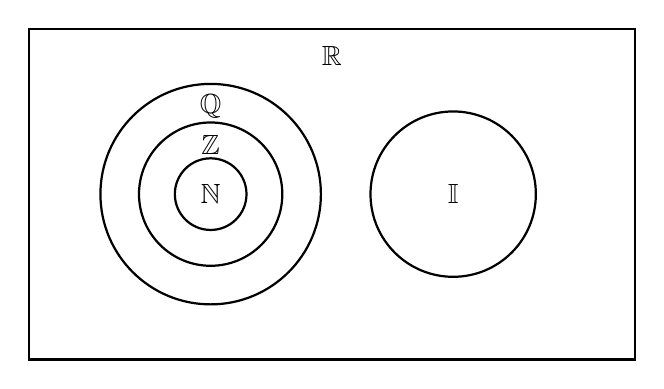
\begin{tikzpicture}[scale=0.7]
    % Real numbers rectangle (outermost)
    \draw[thick] (-5.5,-3) rectangle (5.5,3);
    \node at (0, 2.5) {$\mathbb{R}$};
    
    % Rational numbers circle (left side)
    \draw[thick] (-2.2,0) circle (2cm);
    \node at (-2.2, 1.6) {$\mathbb{Q}$};
    
    % Integers circle
    \draw[thick] (-2.2,0) circle (1.3cm);
    \node at (-2.2, 0.9) {$\mathbb{Z}$};
    
    % Natural numbers circle (innermost)
    \draw[thick] (-2.2,0) circle (0.65cm);
    \node at (-2.2, 0) {$\mathbb{N}$};
    
    % Irrational numbers circle (right side, disjoint)
    \draw[thick] (2.2,0) circle (1.5cm);
    \node at (2.2, 0) {$\mathbb{I}$};
    
\end{tikzpicture}
\captionsetup{width=0.8\textwidth}
\caption{\small{Hierarchy of number sets: Natural numbers ($\mathbb{N}$), Integers ($\mathbb{Z}$), Rationals ($\mathbb{Q}$), Irrationals ($\mathbb{I}$), and Real numbers ($\mathbb{R}$).}}
\label{fig:number_sets}
\end{figure}


From this idea, we need to build $\mathbb{N_F}$, $\mathbb{Z_F}$, $\mathbb{Q_F}$ and $\mathbb{I_F}$ to finall get this $\mathbb{F}$ we want. This will all make sense in the last part of the process, and it is true that it will be a bit of a hussle to construct all of it (specially $\mathbb{I_F}$ from $\mathbb{Q_F}$), but we need to go step by step.


\begin{definition}[$\mathbb{N}_{\mathbb{F}}$ by induction]
Let $\mathbb{F}$ be \textit{the} complete ordered field. Using $1_\mathbb{F}$: multiplicative neutral of $\mathbb{F}$, we declare the following element contruction:

\begin{align*}
&1_\mathbb{F} := 1_\mathbb{F}\\
&2_\mathbb{F} := 1_\mathbb{F} + 1_\mathbb{F}\\
&3_\mathbb{F} := 1_\mathbb{F} + 1_\mathbb{F} + 1_\mathbb{F}\\
\vdots\\
&n_\mathbb{F} := \sum_{1}^{n}{1_F}
\end{align*}

Finally, we define the set:
$$\mathbb{N_F} := \{1_\mathbb{F}, 2_\mathbb{F}, 3_\mathbb{F}, \dots\} = \{n_\mathbb{F}: n \in \mathbb{N} \}$$
\end{definition}

\begin{definition}[$\mathbb{Z}_\mathbb{F}$ by extension]
Within field $\mathbb{F}$, let the following:
\begin{enumerate}
\item $0_\mathbb{F}$: Additive identity
\item $-x$: Additive inverse
\end{enumerate}

We define the set:
$$\mathbb{Z_F} = \{0_\mathbb{F}\} \cup \mathbb{N_F} \cup \{-x_\mathbb{F}, \forall n_\mathbb{F} \in N_\mathbb{F}\}$$
\end{definition}

\begin{definition}[$\mathbb{Q}_\mathbb{F}$ by operation]
Within field $\mathbb{F}$, let the following:
\begin{enumerate}
\item $a \in \mathbb{F}$
\item $b^{-1}$ (multiplicative inverse of $b$) $\in \mathbb{F}$
\end{enumerate} we define the set:
$$\mathbb{Q_F} := \{\frac{a}{b}: a \in \mathbb{Z_F}, b \in \mathbb{N_F}\}$$
\end{definition}

Starting similarly to \cref{th:archimedean} (Archimedean property) we use the inductive approach to reach $\mathbb{N_F}$. Fancy but not complicated at all. Later, we just extend integers in $\mathbb{F}$ to build by $\mathbb{Z_F}$ to conclude defining $\mathbb{Q_F}$ with the result of operating arbitrary elements $a, b \in \mathbb{F}$ as $a.b^{-1}$.

Notice how we only used existent elements from $\mathbb{F}$ computed using the field's operations and nothing else. Is important to mention that you as the reader don't know yet the usage of these new sets, althought we could make a good guess.

Now comes the tricky part for us. One could think that the next steps involve 1. to prove that the irrational (in $\mathbb{F}$) is in fact buildable from $\mathbb{Q_F}$, and 2. to prove that there is a isomorphism between this result and the $\mathbb{R}$ we know.

That won't be the case. If we would go down that path, we would just be creating an arbitrary function $\Phi$ that maps a generic $\mathbb{F}$ with $\mathbb{R}$ perfectly, losing all progress we made constructing these specific sets one by one (for a reason). The real strategy here is to first prove that $\Phi$ exists and \textit{then} to try to extend this function to make it follow all expected properties in the irrationals. Buckle up.

\subsection{Isomorphism in $\mathbb{Q}s$}
\begin{definition}[$\phi$ function]
Let $\phi: \mathbb{Q_F} \rightarrow \mathbb{Q}$ defined as:
$$\phi(\frac{m}{n}) := \frac{m_\mathbb{F}}{n_\mathbb{F}}$$

Where:
\begin{itemize}
\item $m, n \in \mathbb{Q} \ (m \in \mathbb{Z}, n \in \mathbb{Z^+})$
\item $m_\mathbb{F}, n_\mathbb{F} \in \mathbb{Q_F}$
\end{itemize}
\end{definition}

\begin{lemma}\label{le:phi-homomorphism}
$\phi: \mathbb{Q_F} \rightarrow \mathbb{Q}$
$$\phi(\frac{m}{n}) := \frac{m_\mathbb{F}}{n_\mathbb{F}}$$ is an homomorphism
\end{lemma}

\begin{bookproof}
For $m_1/n_1, m_2/n_2 \in \mathbb{Q}$

\begin{enumerate}
\item $\phi(x + y) = \phi(x) + \phi(y)$
\begin{align*}
\phi(m_1/n_1 + m_2/n_2) &= \phi(\frac{m_1.n_2 + m_2.n_1}{n_1.n_2}) \\
&= \frac{(m_1.n_2 + m_2.n_1)_\mathbb{F}}{(n_1.n_2)_\mathbb{F}} \\ 
&= \frac{(m_1.n_2)_\mathbb{F} + (m_2.n_1)_\mathbb{F}}{(n_1)_\mathbb{F}.(n_2)_\mathbb{F}} \\
&= \frac{(m_1)_\mathbb{F}.(n_2)_\mathbb{F} + (m_2)_\mathbb{F}.(n_1)_\mathbb{F}}{(n_1)_\mathbb{F}.(n_2)_\mathbb{F}} \\
&= \frac{(m_1)_\mathbb{F}}{(n_1)_\mathbb{F}} + \frac{(m_2)_\mathbb{F}}{(n_2)_\mathbb{F}} \\\\
\phi(m_1/n_1 + m_2/n_2) &= \phi(m_1/n_1) + \phi(m_2/n_2)
\end{align*}

\item $\phi(x.y) = \phi(x) . \phi(y)$
\begin{align*}
\phi(m_1/n_1 . m_2/n_2) &= \phi(\frac{m_1.m_2}{n_1.n_2}) \\
&= \frac{(m_1.m_2)_\mathbb{F}}{(n_1.n_2)_\mathbb{F}} \\
&= \frac{(m_1)_\mathbb{F}.(m_2)_\mathbb{F}}{(n_1)_\mathbb{F}.(n_2)_\mathbb{F}} \\
&= \frac{(m_1)_\mathbb{F}}{(n_1)_\mathbb{F}} . \frac{(m_2)_\mathbb{F}}{(n_2)_\mathbb{F}} \\\\
\phi(m_1/n_1 . m_2/n_2) &= \phi(m_1/n_1) . \phi(m_2/n_2)
\end{align*}
\end{enumerate}

Finally, $\phi$ is an homomorphism.
\end{bookproof}

Now comes the monster. In order to get the isomorphism, we need to make sure $\phi$ preserves order to prove injectivity by \cref{le:inj-by-order}, and this step alone takes several previous lemmas to cover it fully, and of course we will see them all. Just remember we are having fun.

\begin{lemma}[Ordering in $\mathbb{N_F}$]
For $n, k \in \mathbb{N}, n_\mathbb{F}, k_\mathbb{F} \in \mathbb{N_F}$
\begin{enumerate}
\item If $n < k \rightarrow n_\mathbb{F}< k_\mathbb{F}$
\item If $n = k \rightarrow n_\mathbb{F}= k_\mathbb{F}$
\item If $n > k \rightarrow n_\mathbb{F}> k_\mathbb{F}$
\end{enumerate}
\end{lemma}

\begin{bookproof}
\begin{enumerate}
\item $n = k \rightarrow n_\mathbb{F} = k_\mathbb{F}$

$$n_\mathbb{F} := \sum_{1}^{n}{1_F} = \sum_{1}^{k}{1_F} = n_\mathbb{F}$$

\item $n < k \rightarrow n_\mathbb{F} < k_\mathbb{F}$

$$n < k \Leftrightarrow \exists p \in \mathbb{N}: n + p = k$$

Now, $k_\mathbb{F}$ can be expressed as:
$$k_\mathbb{F} := \sum_{1}^{k}{1_F} = \sum_{1}^{n}{1_F} + \sum_{1}^{p}{1_F}  = n_\mathbb{F} + p_\mathbb{F}$$

Since $p > 1$, using order preservation in addition for fields (\cref{def:ordered-fields}) we have:
$$k_\mathbb{F} = n_\mathbb{F} + p_\mathbb{F} > n_\mathbb{F} + 0_\mathbb{F} > n_\mathbb{F}$$

\item $n > k \rightarrow n_\mathbb{F} > k_\mathbb{F}$

$$n > k \leftrightarrow k < n$$
From 2.
$$n_\mathbb{n} > k_\mathbb{n} $$
\end{enumerate}
\end{bookproof}

\begin{lemma}[Ordering in $\mathbb{Z_F}$]\label{le:ordering-Z}
For $n, k \in \mathbb{Z}, n_\mathbb{F}, k_\mathbb{F} \in \mathbb{Z_F}$
\begin{enumerate}
\item If $n < k \rightarrow n_\mathbb{F}< k_\mathbb{F}$
\item If $n = k \rightarrow n_\mathbb{F}= k_\mathbb{F}$
\item If $n > k \rightarrow n_\mathbb{F}> k_\mathbb{F}$
\end{enumerate}
\end{lemma}

\begin{bookproof}
\begin{enumerate}
\item $n = k \rightarrow n_\mathbb{F} = k_\mathbb{F}$
\begin{enumerate}
\item $n, k >= 0$: Same as the proof for $\mathbb{N_F}$
\item $n, k < 0$: $$n = k \leftrightarrow -k = -n \rightarrow -k, -n \in \mathbb{N}$$
\end{enumerate}
We now proceed exactly as the proof for $\mathbb{N_F}$

\item $n < k \rightarrow n_\mathbb{F} < k_\mathbb{F}$, similarly to $\mathbb{N_F}$:
\begin{align*}
n < k \Leftrightarrow \exists p \in \mathbb{N}: n + p = k
\end{align*}

\begin{enumerate}
\item $n >= 0$: Since $n \in \mathbb{N} \rightarrow (n + p)_\mathbb{F} = n_\mathbb{F} + p_\mathbb{F}$

\item $n < 0$: Labeling $n = -t$ just to indicate it is negative by sign:
\begin{align*}
&\rightarrow n = -t \leftrightarrow n_\mathbb{F} = -t_\mathbb{F} \wedge (-t) + p = k \\
&\rightarrow p = k + t \\
&\rightarrow p_\mathbb{F} = k_\mathbb{F} + t_\mathbb{F} \\
&\rightarrow p_\mathbb{F} = k_\mathbb{F} - n_\mathbb{F} \\
&\rightarrow n_\mathbb{F} + p_\mathbb{F} = k_\mathbb{F} \\
&\rightarrow n_\mathbb{F} + p_\mathbb{F} = k_\mathbb{F} = (n + p)_\mathbb{F}
\end{align*}
Therefore, we prooved for any case of $n, k \in \mathbb{Z}: n < k \rightarrow n_\mathbb{F} < k_\mathbb{F}$
\end{enumerate}

\item $n > k \rightarrow n_\mathbb{F}> k_\mathbb{F}$
\\\\
Labeling acrodingly: $n > k \leftrightarrow -n^\prime > -k^\prime \leftrightarrow n^\prime < k^\prime (n^\prime, k^\prime \in \mathbb{N})$\\
With this we just proceed as in 2
\end{enumerate}
\end{bookproof}

So far so \textquotedblleft good\textquotedblright. Now, before moving to $\mathbb{Q}$ we need an extra tool for operating multiplications in $\mathbb{Z_F}$.

\begin{lemma}[Multiplication in $\mathbb{Z_F}$]\label{le:mult-in-Z}
For any $n, k \in \mathbb{Z}$ \\
$$(n.k)_\mathbb{F} = n_\mathbb{F} . k_\mathbb{F} \in \mathbb{F}$$
\end{lemma}

\begin{bookproof}
\begin{enumerate}
\item $n, k > 0:$\\\\
We have:
$$(n . k)_\mathbb{F} = \sum_{1}^{n.k} 1_\mathbb{F} = \sum_{1}^{n} \sum_{1}^{k} 1_\mathbb{F} =  \sum_{1}^{n} k_\mathbb{F} = n_\mathbb{F} . k_\mathbb{F}$$
Which is just adding the additive neutral $n.k$ times.


\item $n > 0, k < 0:$ \\\\
Writing $k$ as $-m$ to denote negativeness, we have:
$$(n.k)_\mathbb{F} = (n(-m))_\mathbb{F} = (-n.m)_\mathbb{F} = -(n.m)_\mathbb{F}$$
From 1:
$$(n.k)_\mathbb{F} = -n_\mathbb{F}.m_\mathbb{F} = n_\mathbb{F}.-m_\mathbb{F} = n_\mathbb{F}.k_\mathbb{F}$$
\end{enumerate}
\end{bookproof}

\begin{lemma}[Ordering in $\mathbb{Q}$]\label{le:ordering-Q}
Let $\frac{m_1}{n_1}, \frac{m_2}{n_2} \in \mathbb{Q}$ \\
$$\frac{m_1}{n_1} < \frac{m_2}{n_2} \rightarrow (\frac{m_1}{n_1})_\mathbb{F} < (\frac{m_2}{n_2})_\mathbb{F}$$
\end{lemma}

\begin{bookproof}
Arbitrary locking $n_1, n_2 \in \mathbb{N}$ without losing generalization, we have:
$$\frac{m_1}{n_1} < \frac{m_2}{n_2} \leftrightarrow m_1.n_2 < m_2.n_1$$
Maintaing the inequality direction
Now, from \cref{le:ordering-Z}:
$$m_1.n_2 < m_2.n_1 \leftrightarrow (m_1.n_2)_\mathbb{F} < (m_2.n_1)_\mathbb{F}$$
Next, from \cref{le:mult-in-Z}:
$$(m_1.n_2)_\mathbb{F} < (m_2.n_1)_\mathbb{F} \leftrightarrow (m_1)_\mathbb{F}.(n_2)_\mathbb{F} < (m_2)_\mathbb{F}.(n_1)_\mathbb{F}$$
Now, since we fixed $n1, n2 \in \mathbb{N}$, we can use $(n1.n2)_\mathbb{F}$ to divide the expression:
$$(m_1)_\mathbb{F}.(n_2)_\mathbb{F} < (m_2)_\mathbb{F}.(n_1)_\mathbb{F} \leftrightarrow \frac{(m_1)_\mathbb{F}.(n_2)_\mathbb{F}}{(n_1.n_2)_\mathbb{F}} . \frac{(m_2)_\mathbb{F}.(n_1)_\mathbb{F}}{(n_1.n_2)_\mathbb{F}}$$
Next, we just distribute and simplify:
$$\frac{(m_1)_\mathbb{F}.(n_2)_\mathbb{F}}{(n_1.n_2)_\mathbb{F}} . \frac{(m_2)_\mathbb{F}.(n_1)_\mathbb{F}}{(n_1.n_2)_\mathbb{F}} \leftrightarrow \frac{(m_1)_\mathbb{F}}{(n_1)_\mathbb{F}} . \frac{(m_2)_\mathbb{F}}{(n_1)_\mathbb{F}}$$

Finally, we have:
$$\frac{m_1}{n_1} < \frac{m_2}{n_2} \leftrightarrow \frac{(m_1)_\mathbb{F}}{(n_1)_\mathbb{F}} . \frac{(m_2)_\mathbb{F}}{(n_1)_\mathbb{F}}$$
\\
$$\frac{m_1}{n_1} < \frac{m_2}{n_2} \leftrightarrow (\frac{m_1}{n_1})_\mathbb{F} < (\frac{m_2}{n_2})_\mathbb{F}$$
\end{bookproof}

Now if we recall, we did all of this as a previous step for proving the injectivity of $\phi$. We can make it happen now.

\begin{lemma}\label{le:phi-injective}
$\phi: \mathbb{Q_F} \rightarrow \mathbb{Q}$
$$\phi(\frac{m}{n}) := \frac{m_\mathbb{F}}{n_\mathbb{F}}$$ is injective
\end{lemma}

\begin{bookproof}
Let $\frac{m_1}{n_1}, \frac{m_2}{n_2} \in \mathbb{Q}$, such that:

$$\frac{m_1}{n_1} < \frac{m_2}{n_2}$$

By \cref{le:ordering-Q}, we have:

$$\frac{m_1}{n_1} < \frac{m_2}{n_2} \rightarrow (\frac{m_1}{n_1})_\mathbb{F} < (\frac{m_2}{n_2})_\mathbb{F}$$

By definition of $\phi$, we can replace:

\begin{align*}
\frac{m_1}{n_1} < \frac{m_2}{n_2} &\rightarrow \frac{(m_1)_\mathbb{F}}{(n_1)_\mathbb{F}} < \frac{(m_2)_\mathbb{F}}{(n_2)_\mathbb{F}} \\\\
\frac{m_1}{n_1} < \frac{m_2}{n_2} &\rightarrow \phi(\frac{m_1}{n_1}) < \phi(\frac{m_1}{n_1}) \\
\end{align*}
$$\Rightarrow \phi : \mathbb{Q} \rightarrow \mathbb{Q_F} \text{ preserves order.}$$ \\

Finally, from \cref{le:inj-by-order} (Injectivity by order preservation) we assert:\\

$$\Rightarrow \phi : \mathbb{Q} \rightarrow \mathbb{Q_F} \text{ is injective.}$$
\end{bookproof}

\begin{lemma}\label{le:phi-surjective}
$\phi: \mathbb{Q_F} \rightarrow \mathbb{Q}$
$$\phi(\frac{m}{n}) := \frac{m_\mathbb{F}}{n_\mathbb{F}}$$ is surjective
\end{lemma}

\begin{bookproof}
By set construction (\cref{le:sur-by-construction}) we defined $\phi: \mathbb{Q_F} \rightarrow \mathbb{Q}$, meaning that:
$$\mathbb{Q} = Im(\mathbb{Q_F})$$
Then
$$\phi \text{ is surjective.}$$
\end{bookproof}

This completes the construction.

\begin{lemma}
$\phi: \mathbb{Q_F} \rightarrow \mathbb{Q}$
$$\phi(\frac{m}{n}) := \frac{m_\mathbb{F}}{n_\mathbb{F}}$$ is an isomorphism
\end{lemma}

\begin{bookproof}
\begin{enumerate}
\item By \cref{le:phi-homomorphism}, $\phi$ is an homomorphism.
\item By \cref{le:phi-injective} and \cref{le:phi-surjective}, $\phi$ is bijective
\end{enumerate}
Then, by \cref{def:field-isomorphism}

$$\Rightarrow \phi \text{ is an isomorphism}.$$
\end{bookproof}

Securing this is a big step, and recalling our strategy we now need to use this isomorphism $\phi$ in $\mathbb{Q_F} \rightarrow \mathbb{Q}$, and somehow transform it into a $\Phi$ that extends this to the whole $\mathbb{F} \rightarrow \mathbb{R}$.

Although this has being a long ride, personally I don't think this was a complex construction, or a hard-to-follow implementation of $\phi$. Everything just landed in place.

The tricky part begins when we introduce $\Phi$ and try to understand what it really is. Still, I wouldn’t include anything that I wouldn’t find clear or satisfactory from a student’s perspective (keep in mind I'm also learning while writing). If something feels confusing or lacks intuition, I prefer to leave it out entirely and try again.

\subsection{Isomorphism in $\mathbb{R}$}
We have successfully constructed an isomorphism $\phi: \mathbb{Q_F} \rightarrow \mathbb{Q}$ that preserves all the important conditions (order, addition and multiplication), but our main goal is to extend this to all $\mathbb{R}$, starting from all $\mathbb{F}$.

So we expect a:
$$\Phi: \mathbb{F} \rightarrow \mathbb{R}$$

Such that:

\begin{enumerate}
\item Matches the former $\phi$ for all $\mathbb{Q_F}$ into $\mathbb{Q}$
\item Remains an isomorphism
\item Preserves the field's struture (order, addition and multiplication)
\end{enumerate}

The intuiton to create $\Phi$ was actually mentioned previously, on \cref{ex:s-in-q-not-bounded}. We talked about how a subset $S$ of an ordered field $\mathbb{Q}$ was bounded above by $\sqrt{2}$. The example talks more about how this $S$ won't have a supremum, but the key idea we will be using is how this particular $S$ was \textbf{bounded} by an irrational like $\sqrt{2}$. This is the relationship we need to apply to link irrational and rational numbers: \textbf{the first one bounds the second one}

With this idea, we can intuit that any \textbf{real number is actually defined by the numbers below it}. Take $\sqrt{2}$ for example:

\begin{enumerate}
\item $\sqrt{2}$ is greater than all the rationals $q$ where $q < \sqrt{2}$: 1, 1.4, 1.41, 1.414, \dots
\item $\sqrt{2}$ is less than all the rationals $q$ where $q > \sqrt{2}$: 2, 1.5, 1.42, 1.4145, \dots
\end{enumerate}

The fact is that $\sqrt{2}$ is the only number placed in the boundary between these to sequences.

More formally:
$$\sqrt{2} := \sup \{q \in \mathbb{Q}: q < \sqrt{2}\}$$
Relating an irrational number, with all the rationals below it.

\begin{definition}[$\Phi$ function]\label{def:Phi-function}
For any $\alpha \in \mathbb{R}$, define $\Phi: \mathbb{R} \rightarrow \mathbb{F}$ as
$$\Phi(\alpha) := \sup\{\phi(q): q \in \mathbb{Q}, q < \alpha \}$$
\end{definition}

This new function $\Phi$ using the former isomorphism $\phi$ defined in $\mathbb{Q}$ does the exact same thing that $\sqrt{2}$ did in our example: bounds $\mathbb{Q}$. Since our main focus is to somehow extend the properties of the original $\phi$, lets take the time to emphazise why this new $\Phi$ is not just an arbitrary function.

\begin{lemma}
For $r \in \mathbb{Q}$
\begin{align*}
\Phi(r)  = \phi(r)
\end{align*}
\end{lemma}

\begin{bookproof}
First, lets check the definition:
$$\Phi(\alpha) := \sup\{\phi(q): q \in \mathbb{Q}, q < \alpha \}$$

If $\alpha$ happens to be a rational number $r$, it means that the supremum of all the rational values before this particular $r$ are limited by $\phi(r)$, and this is the \textit{Least Upper Bound} of the set.

\begin{enumerate}
\item $\phi(r)$ bounds $\{\phi(q): q \in \mathbb{Q}, q < r \}$\\\\
Knowing that $\phi$ preserves order:
\begin{align*}
\forall q, q < r &\leftrightarrow \phi (q) < \phi (r)\\
&\leftrightarrow \phi(q) \leq \phi(r)
\end{align*}
$\Rightarrow \phi(r)$ bounds the set.
\end{enumerate}
\end{bookproof}

\begin{bookproof}
\begin{enumerate}
\setcounter{enumi}{1}
\item $\phi(r)$ is the L.U.B. of $\{\phi(q): q \in \mathbb{Q}, q < r \}$
\\\\
Lets visualize the approach

\begin{figure}[H]
\centering
\small
\begin{tikzcd}[column sep=scriptsize, row sep=small, scale=0.85]
	&&&&&&&&& {\textit{LUB}} \\
	{\mathbb{Q}} & {q_1} & {q_2} & \dots & q && {} & {q^\prime} & r & {} \\
	\\
	\\
	{\mathbb{Q}_F} & {\phi(q_1)} & {\phi(q_2)} & \dots & {\phi(q)} && M & {\phi(q^\prime)} & {\phi(r)} & {} \\
	&&&&& {} &&&& {}
	\arrow[shift right=4, from=2-1, to=2-10]
	\arrow["\phi"{description}, Rightarrow, from=2-1, to=5-1]
	\arrow[from=2-2, to=5-2]
	\arrow[from=2-3, to=5-3]
	\arrow[from=2-5, to=5-5]
	\arrow["{{\epsilon_M/2}}"{description}, shift left=5, between={0.3}{0.7}, no head, from=2-7, to=2-10]
	\arrow[from=2-8, to=5-8]
	\arrow[shift left=2, curve={height=18pt}, between={0}{0.9}, from=2-9, to=1-10]
	\arrow[from=2-9, to=5-9]
	\arrow[shift left=4, from=5-1, to=5-10]
	\arrow["{{\epsilon_M}}"{description}, shift left=2, between={0.2}{0.8}, no head, from=6-6, to=6-10]
\end{tikzcd}
\end{figure}


Assume $M$ is an arbitrary upper bound, trying to make $\phi(r)$ not the \textit{L.U.B.}
\begin{align*}
\rightarrow M < \phi(r)
\rightarrow \phi(r) - M > 0
\end{align*}
Lets call $\epsilon_M$ to the distance between this assumed $M$ and $\phi(r)$.

Now, lets not forget that by density in $\mathbb{Q}$ we are able to locate an arbitrary rational number between two other arbitrary rationals, or even better for our use case: we can position an arbitrary rational $q^\prime$ as close as we want to any other arbitrary rational.

Developing that idea:
\begin{align*}
\forall \ r \in \mathbb{Q}, \exists \ q^\prime \in \mathbb{Q} : q^\prime - \epsilon \leq r, \epsilon \in \mathbb{Q}
\end{align*}

Now, $M \in \mathbb{Q_F}$, but the density propery we are using for $q^\prime$ is in $\mathbb{Q}$. Luckily, we already proved that $\phi$ is ordered:


\begin{align*}
\forall \ r \in \mathbb{Q}&, \exists \ q^\prime \in \mathbb{Q} / \forall \epsilon > 0: q^\prime - \epsilon \leq r \\
&\rightarrow \phi(q^\prime) - \phi(\epsilon) \leq \phi(r)
\end{align*}

Now that we are entirely in $\mathbb{Q_F}$ we will conveniently take this distance $\phi(\epsilon)$ as $\epsilon_M / 2$, just to note that this will be smaller than the distance between $M$ and $r$. No matter how close we assume $M$ is to $\phi(r)$, by density in $\mathbb{Q}$ we can make sure that we can take half that distance (or a quarter, or a tenth, doesn't matter) to locate another image closer to $\phi(r)$.

\begin{align*}
\rightarrow M < \phi(q^\prime) < \phi(r)
\rightarrow M \neq \text{ Upper bound}
\end{align*}
$$\Rightarrow \Phi(r) := \sup\{\phi(q): q \in \mathbb{Q}, q < r \} = \phi(r), \ \forall r \in \mathbb{Q}$$
\end{enumerate}
\end{bookproof}	

Taking the time to proof this mapping for rationals wasn't a waste of time after all, since it confirms that our intuition about the definition of $\Phi$ isn't arbitrary, but respects the structure we already built.


\subsubsection{Completeness of $\Phi$}

So far, our definition for $\Phi$:

$$\Phi(\alpha) := \sup\{\phi(q): q \in \mathbb{Q}, q < \alpha \}$$

Uses an internal set $S(\alpha) = \{\phi(q): q \in \mathbb{Q}, q < \alpha \}$ that we can use to simplify our readability a bit:

$$\Phi(\alpha) := \sup(S(\alpha))$$

Now, to make $\Phi$ to make sense we need to make sure that $S$ makes sense, and if we want to obtain the supremum of a poorly-define set, the whole definition crumbles.

Next, we will review how $S(\alpha)$ is well defined to avoid any issues further down.

\begin{lemma}
Set $S$:
$$\Phi(\alpha) := \sup\{S(\alpha)\} = \sup\{\phi(q): q \in \mathbb{Q}, q < \alpha \}$$ is well defined in $\mathbb{R}$
\end{lemma}

\begin{bookproof}
To proof this, what matters the most is that $S$ is well-defined in $\mathbb{F}$. That automatically guarantees that $\Phi$ makes sense in $\mathbb{R}$.
\begin{enumerate}
\item $S(\alpha)$ is not empty:

Using \cref{th:archimedean} (Archimedean theorem):
\begin{align*}
&\forall \alpha \in \mathbb{Q}, \exists \ n \in \mathbb{N}: n > \alpha \\
&\rightarrow n > |\alpha| \\
&\rightarrow -n < \alpha, -n \in \mathbb{Q}
\end{align*}
Identifying $q = -n$ in $S$, we have a rational that is bounded by $\alpha$, meaning that $\phi(-n) \in S(\alpha)$
\\
\item $S(\alpha)$ is bounded above:

Again, using \cref{th:archimedean}:
\begin{align*}
&\forall \alpha \in \mathbb{Q}, \exists \ n \in \mathbb{N}: n > \alpha \\
\end{align*}
Then, for any rational $q < \alpha$
\begin{align*}
& n > \alpha > q \\
& \rightarrow q < n \\
& \rightarrow \phi(q) < \phi(n) = n_\mathbb{F}\\
\end{align*}
So $n_\mathbb{F}$ is an upper bound of $S$, for any $q < \alpha$
\end{enumerate}
$\rightarrow S(\alpha)$ is well-defined in $\mathbb{F}$ \\\\
$\rightarrow \Phi(\alpha) := \sup\{S(\alpha)\}$ is well-defined in $\mathbb{R}$
\end{bookproof}

Now, while studying this a question came to me: if we already know that $\phi: \mathbb{Q} \rightarrow \mathbb{Q_F}$ exists, why do we need to prove $S(\alpha)$ is non-empty? Can't we just pick any rational and map it?


The issue is that the set $S(\alpha)$ is not just any images of rationals, it's specifically:
$S(\alpha) = \{\phi(q) : q \in \mathbb{Q} \text{ AND } q < \alpha\}$. The constraint $q < \alpha$ obligues us to prove that \textit{there exists at least one rational $q$ with $q < \alpha$}.

\begin{lemma}[Order-Preservation]\label{le:order-Phi}
For $\alpha, \beta \in \mathbb{R}$

$$\alpha < \beta \rightarrow \Phi(\alpha) < \Phi(\beta)$$
\end{lemma}

\begin{bookproof}
Lets start with two evaluations of set $S$:
\begin{itemize}
\item $S(\alpha) := \{\phi(q): q \in \mathbb{Q}, q < \alpha \}$
\item $S(\beta) := \{\phi(q): q \in \mathbb{Q}, q < \beta \}$
\end{itemize}

If $\alpha < \beta$, then for any $\phi(q^\prime) \in S(\alpha)$:
\begin{align*}
\phi(q) \in S(\alpha) &\leftrightarrow \phi(q^\prime) \in \{\phi(q): q \in \mathbb{Q}, q < \alpha \} \\
&\leftrightarrow \phi(q^\prime) \in \{\phi(q): q \in \mathbb{Q}, q < \alpha < \beta \} \\
&\leftrightarrow \phi(q^\prime) \in \{\phi(q): q \in \mathbb{Q}, q < \beta \} \\
&\leftrightarrow \phi(q^\prime) \in S(\beta)
\end{align*}

Then, going back to the statement:

\begin{align*}
\alpha < \beta &\Rightarrow S(\alpha) \subseteq S(\beta) \\
&\Rightarrow \sup(S(\alpha)) \leq \sup(S(\beta)) \\
&\Rightarrow \Phi(\alpha) \leq \Phi(\beta)
\end{align*}

Now, to prove that the images of $\alpha$ and $\beta$ in $\Phi$ are strictly less than and not equal, we use the density of $\mathbb{Q}$ in $\mathbb{R}$ to locate arbitrary rationals $r_\alpha, r_\beta$.
\begin{align*}
\forall \alpha, \beta \in \mathbb{R}, \exists \ r_\alpha, r_\beta \in \mathbb{Q}: \\
\alpha < \beta \rightarrow  \alpha < r_\alpha < r_\beta < \beta \\
\end{align*}

Since $r_\beta < \beta \rightarrow \phi(r_\beta) \in S(\beta)$ by the definition of $S$. Now, knowing that for any element of $S(\beta)$ it will be less or equal to its supremum, we have:
\begin{align*}
\phi(r_\beta) \leq \sup(S(\beta)) \\
\phi(r_\beta) \leq \Phi(\beta)
\end{align*}

Now in the middle, by order preservation:
\begin{align*}
r_\alpha < r_\beta \leftrightarrow \phi(r_\alpha) < \phi(r_\beta)
\end{align*}

And finally, since $\alpha < r_\alpha \rightarrow S(\alpha) \subseteq S(r_\alpha)$. Then:

\begin{align*}
&S(\alpha) \subseteq S(r_\alpha) \\
&\rightarrow \Phi(\alpha) \leq \Phi(r_\alpha) \\
&\rightarrow \Phi(\alpha) \leq \phi(r_\alpha) \text{ (Since $r_\alpha \in \mathbb{Q}$)} \\
\end{align*}

Joining all results:
\begin{align*}
\Phi(\alpha) &\leq \phi(r_\alpha) < \phi(r_\beta) \leq \Phi(\beta) \\
&\Rightarrow \Phi(\alpha) < \Phi(\beta) \\
\end{align*}

Finally, $\alpha < \beta \Rightarrow \Phi(\alpha) < \Phi(\beta)$.
\end{bookproof}

Now comes the final sprint to proof that $\Phi$ maps $\mathbb{F}$ and $\mathbb{R}$ perfectly. Just as we did with $\phi$, we need to prove isomorphism by proving bijection and homomorphism. From this last part, the only tricky step is for surjectiveness, since it uses a method that we haven't seeing before. We are almost there!

\begin{lemma}[Injectivity in $\Phi$]
Given $\Phi: \mathbb{R} \rightarrow \mathbb{F}$
, for $\alpha, \beta \in \mathbb{R}:$
$$\alpha \neq \beta \rightarrow \Phi(\alpha) \neq \Phi(\beta)$$
\end{lemma}

\begin{bookproof}
From proven order preservation in \cref{le:order-Phi}, if $\alpha \neq \beta$
\begin{enumerate}
\item $\alpha < \beta \rightarrow \Phi(\alpha) < \Phi(\beta) \rightarrow \Phi(\alpha) \neq \Phi(\beta)$
\item $\alpha > \beta \rightarrow \Phi(\alpha) > \Phi(\beta) \rightarrow \Phi(\alpha) \neq \Phi(\beta)$ 
\end{enumerate}
\end{bookproof}

\begin{lemma}[Surjectivity in $\Phi$]
Given $\Phi: \mathbb{R} \rightarrow \mathbb{F}$:
$$\forall \  a \in \mathbb{F},\exists \ \alpha \in \mathbb{R}: \Phi(\alpha) = a$$
\end{lemma}

\begin{bookproof}
Lets support the following ideas on the next diagram:
\begin{center}
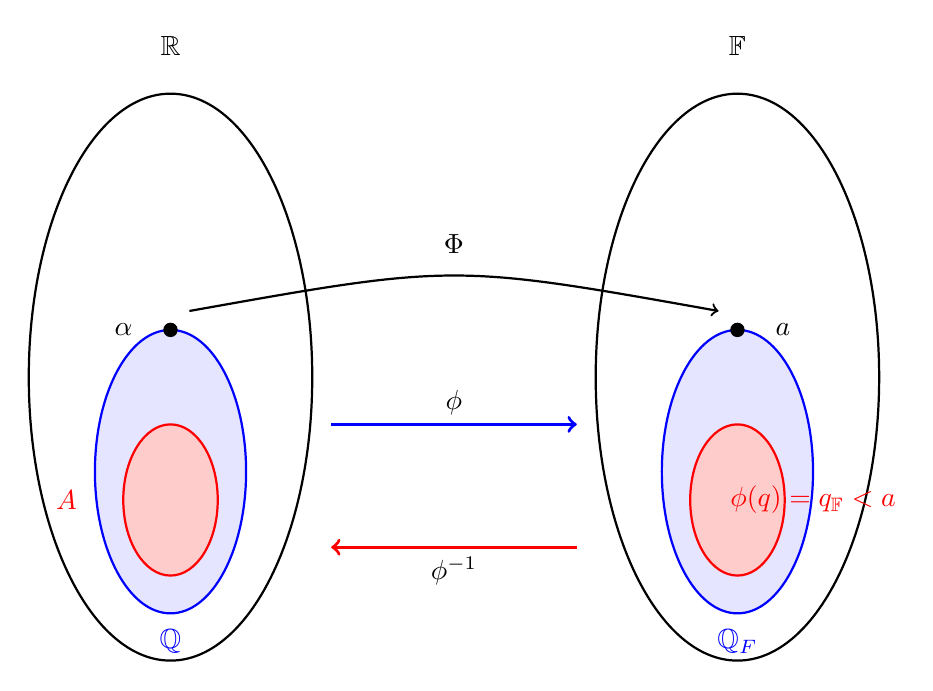
\begin{tikzpicture}[scale=1.2]
    % Left set (R)
    \draw[thick] (-2,0) ellipse (1.5cm and 3cm);
    \node at (-2, 3.5) {$\mathbb{R}$};
    
    % Right set (F)
    \draw[thick] (4,0) ellipse (1.5cm and 3cm);
    \node at (4, 3.5) {$\mathbb{F}$};
    
    % Rationals in R (highlighted region)
    \draw[thick, blue, fill=blue!10] (-2,-1) ellipse (0.8cm and 1.5cm);
    \node[blue] at (-2, -2.8) {$\mathbb{Q}$};
    
    % Rationals in F (highlighted region)
    \draw[thick, blue, fill=blue!10] (4,-1) ellipse (0.8cm and 1.5cm);
    \node[blue] at (4, -2.8) {$\mathbb{Q}_F$};
    
    % Set A (the preimage)
    \draw[thick, red, fill=red!20] (-2,-1.3) ellipse (0.5cm and 0.8cm);
    \node[red] at (-3.1, -1.3) {$A$};
    
    % Elements below a in Q_F
    \draw[thick, red, fill=red!20] (4,-1.3) ellipse (0.5cm and 0.8cm);
    \node[red] at (4.8, -1.3) {$\phi(q) = q_\mathbb{F} < a$};
    
    % Alpha (supremum of A)
    \filldraw[black] (-2, 0.5) circle (2pt);
    \node[left] at (-2.3, 0.5) {$\alpha$};
    
    % a in F
    \filldraw[black] (4, 0.5) circle (2pt);
    \node[right] at (4.3, 0.5) {$a$};
    
    % Phi arrow (forward)
    \draw[->, very thick, blue] (-0.3, -0.5) -- (2.3, -0.5);
    \node[above] at (1, -0.5) {$\phi$};
    
    % Phi inverse arrow (backward)
    \draw[->, very thick, red] (2.3, -1.8) -- (-0.3, -1.8);
    \node[below] at (1, -1.8) {$\phi^{-1}$};
    
    % Phi arrow from alpha to a
    \draw[->, thick, black] (-1.8, 0.7) .. controls (1, 1.2) .. (3.8, 0.7);
    \node[above] at (1, 1.2) {$\Phi$};
\end{tikzpicture}
\end{center}


Picking an arbitrary $a \in \mathbb{Q_F}$, we define the subset bounded above by this $a$:
$$\{\phi(q) = q_\mathbb{F} \in \mathbb{Q_F}, q_\mathbb{F} < a\}$$

Now, since we already know that $\phi$ is a isomorphism (and hence, is injective), we know that its inverse $\phi ^{-1}$ exists. Applying it to the defined set we create $A$:

\begin{align*}
A &= \phi ^{-1}(\{q_\mathbb{F} \in \mathbb{Q_F}, q_\mathbb{F} < a\}) \\
&= \phi ^{-1}(\{\phi(q), q \in \mathbb{Q}, \phi(q) < a\}) \\
&= \{q \in \mathbb{Q}, \phi(q) < a\})
\end{align*}

Now lets consider $\alpha = \sup(A)$, lets first prove that $\alpha$ exists:

\begin{enumerate}
\item $A$ is non-empty:

Let an arbitrary $q \in \mathbb{Q}$, then $\phi(q) = q_\mathbb{F} \in \mathbb{Q_F}$. This means that $\phi(q) < a$, and by definition of $A$, $q \in A$.

\item $A$ is bounded above:

Using the archimedean property in $\mathbb{F}: \exists n_\mathbb{F} \in \mathbb{N_\mathbb{F}}: n_\mathbb{F} > a$. But from the definition of $A, \exists q \in \mathbb{Q}: \phi(q) < a$. Then $\phi(a) < a < n_\mathbb{F}$. Since $\phi$ is order-preserving, we evaluate its inverse in the interval and get $\phi^{-1}(\phi(a)) < \phi^{-1}(n_\mathbb{F})$. Then, $a < n$ shows that $n$ is an upper bound for $A$.
\end{enumerate}

$\Rightarrow \alpha = \sup(A)$ exists
\end{bookproof}

\begin{bookproof}
Now, want we want to achieve is that given this arbitrary $a$, we reach the preimage $\alpha$ by expanding se $A$ enough to declare that $\alpha$ is its supremum. That way, we match the definition of $\Phi$ and that would be it.
\\\\
Claim: $$\{q \in \mathbb{Q}: q < \alpha\} = A$$

\begin{itemize}
\item $\subseteq$:

Let $q \in \mathbb{Q}: q < \alpha$. If we fix an arbitrary $q^\prime \in A$ and using the fact that $\alpha = \sup(A)$, then there is an $\epsilon$ small enough (the minimal in fact) that $q^\prime + \epsilon > \alpha$. Now, ordering:

\begin{align*}
&q < q^\prime < \alpha &\text{ (choosing the smallest $\epsilon$)} \\
&\rightarrow q < q^\prime \\
&\rightarrow \phi(q) < \phi(q^\prime) &\text{ (due $\phi$ preserving order)}
\end{align*}

Since $\phi(q^\prime) \in \mathbb{Q_F}$, $\phi(q^\prime) < a$ (as the diagram implies from our initial assumptions)

$$\rightarrow \phi(q) < \phi(q^\prime) < a$$
$$\rightarrow q \in A$$

\item $\supseteq$:

Let $q \in A$. By definition, $\phi(q) < a$ and, since $\alpha = \sup(A), q < \alpha$.

$$\rightarrow q \in \{q \in \mathbb{Q}: q < \alpha\}$$
\end{itemize}

$$\Rightarrow \{q \in \mathbb{Q}: q < \alpha\} = A$$

So far we proved that:
\begin{enumerate}
\item $\sup(A) = \alpha$ exists
\item $A = \{q \in \mathbb{Q}: q < \alpha\}$
\end{enumerate}

Lets combine the two:

$$
\sup(A) = \sup\{q \in \mathbb{Q}: q < \alpha\}
$$

And from the definition:
\begin{align*}
\Phi(\alpha) &= \sup\{\phi(q), q \in \mathbb{Q}, q < \alpha\} \\
&= \sup\{\phi(q), q \in A\} \\
\end{align*}

But from the original definition of $A = \phi ^{-1}(\{q_\mathbb{F} \in \mathbb{Q_F}, q_\mathbb{F} < a\})$, and replacing:

\end{bookproof}


\end{document}
